\documentclass[a4paper, 12pt]{article}
\usepackage{graphicx}
\usepackage{verbatim}
% \usepackage{lstlisting}
\usepackage{subfig}
\usepackage{float}
% \usepackage{spanish}   ver bien como es

\begin{document}
\begin{center}
\section*{Aclaraciones Generales}
\end{center}

\newpage
\begin{center}
\section*{Ejercicio 1: Matching M\'aximo}
\end{center}
 
\section*{Introducci\'on}
En este ejercicio se ped\'ia encontrar el matching m\'aximo dentro de un grafo. Se define como matching a un subconjunto de aristas que no comparten v\'ertices. Si bien este ejercicio podr\'ia ser de gran complejidad, el mismo se encuentra en una presentaci\'on mas accesible dado que no hay que aplicar el algoritmo sobre cualquier tipo de grafos, sino que solamente tiene que ser aplicable a grafos de 3 o m\'as nodos que sean ciclos simples, es decir, grafos que en su isomorfismo planar sean simplemente un dibujo de un pol\'igono.

% aca podria ir algun dibujo de como serian los grafos a ver y como seria algun grafo que no hay que analizar.

\section*{Algoritmo}



El algoritmo propuesto como resolucion del problema consiste en transformar el grafo en un vector, dado que al poder ser representado como un pol\'igono, se puede ver que, quitando una sola arista, el grafo se convierte en una sucesi\'on de aristas con peso, lo cual se puede representar con un vector de n\'umeros. La idea del algoritmo es poder encontrar el m\'aximo matching posible, una primera aproximaci\'on a la soluci\'on final, podr\'ia ser la siguiente:

\begin{enumerate}
\item Se toma una arista cualquiera para comenzar. Luego, el matching buscado tiene dos opciones: contener esa arista, o no contenerla. Entonces el resultado ser\'a el m\'aximo entre el matching m\'aximo del grafo sin esa arista(no se utiliza la primer arista tomada) y el matching m\'aximo del grafo sin esa arista, ni ninguno de sus dos aristas vecinas, m\'as el valor de la arista elegida en primer t\'ermino(si se utiliza la primer arista tomada). De esta manera, el problema sobre un grafo, se convierte en 2 problemas similares pero sobre vectores.
\item En este momento, se necesita sacar el matching m\'aximo, pero sobre vectores, para hacer esto se piensa de manera parecida al punto anterior comenzando con el \'ultimo elemento: o bien el matching m\'aximo lo contiene, o bien no lo contiene. Luego, el matching buscado para el vector, sera el m\'aximo entre el matching m\'aximo del vector sin el \'ultimo elemento(caso en el que no se usa el \'ultimo elemento) y el matching m\'aximo del vector sin los \'ultimos dos elementos m\'as el valor del \'ultimo elemento(caso en el que si se utiliza el \'ultimo).

	$matchingMaximo(v_1,v_2,..,v_n) = maximo(matchingMaximo(v_1,v_2,..,v_{n-1}), matchingMaximo(v_1,v_2,..,v_{n-2}) + v_n)$
\item De esta manera, se puede ver que el problema se torna recursivo, siendo solucionado mediante la t\'ecnica de dividir y conquistar, teniendo como caso base los vectores de dos o un elemento resolubles trivialmente.
\end{enumerate}

Si bien el algoritmo propuesto retorna el valor esperado, la complejidad del mismo no es \'optima. Al hacer los llamados recursivos sucede que hay varios matching m\'aximos que se realizan sobre los mismos vectores, generando as\'i m\'as c\'alculos de los necesarios. Fue por esto, que el siguiente paso fue modificar el algoritmo para que no calcule las cosas de modo \emph{top down}, sino que fuese un algoritmo \emph{bottom up}, para as\'i evitar los c\'alculos repetidos, utilizando as\'i la mayor ventaja de la programaci\'on din\'amica, t\'ecnica que define al algoritmo final.

De esta manera, se pens\'o como teniendo instancias m\'as peque~{n}as del problema, se puede conocer la soluci\'on de una instancia mayor. Se utiliz\'o que, dadas las soluciones \'optimas para vectores de n-2 y n-1 elementos, la soluci\'on para el vector de n elementos es el m\'aximo entre la solucion de n-1 elementos, y la soluci\'on de n-2 elementos m\'as el elemento n-\'esimo. Es as\' que el c\'alculo se torna \emph{bottom up}, calculando los m\'aximos de los subvectores, una sola vez.

A continuaci\'on se muestra el pseudoc\'odigo del algoritmo propuesto como resoluci\'on del problema.


% \begin{lstlisting}
\begin{verbatim}
matchingMaximo(grafo G)
   tomar v una arista cualquiera
   tomar u y w vecinos de v
   res := max(matchingSobreVector(G-u-v-w) + v, matchingSobreVector(G-v))

matchingSobreVector(Vector peso_arista)
si tamanio(peso_arista) = 0
   devolver 0
si tamanio(peso_arista) = 1
   devolver peso_arista[1]
si tamanio(peso_arista) = 2
   devolver max(peso_arista[1], peso_arista[2])
si tamanio(peso_arista) >= 3
   peso_maximo_hasta_i-1 := max(peso_arista[1], peso_arista[2]) 
   peso_maximo_hasta_i-2 := peso_arista[1]
   Para i = 3 hasta n {
      temp := peso_maximo_hasta_i-1
      peso_maximo_hasta_i-1 := 
         max( peso_maximo_hasta_i-2 + peso_arista[i], peso_maximo_hasta_i-1)
      peso_maximo_hasta_i-2 := temp
   }
   devolver peso_maximo_hasta_i-1

\end{verbatim}
% \end{lstlisting}

A continuaci\'on se presenta un seguimiento del algoritmo sobre un ciclo simple de siete aristas.

\begin{figure}[H]
\begin{center}
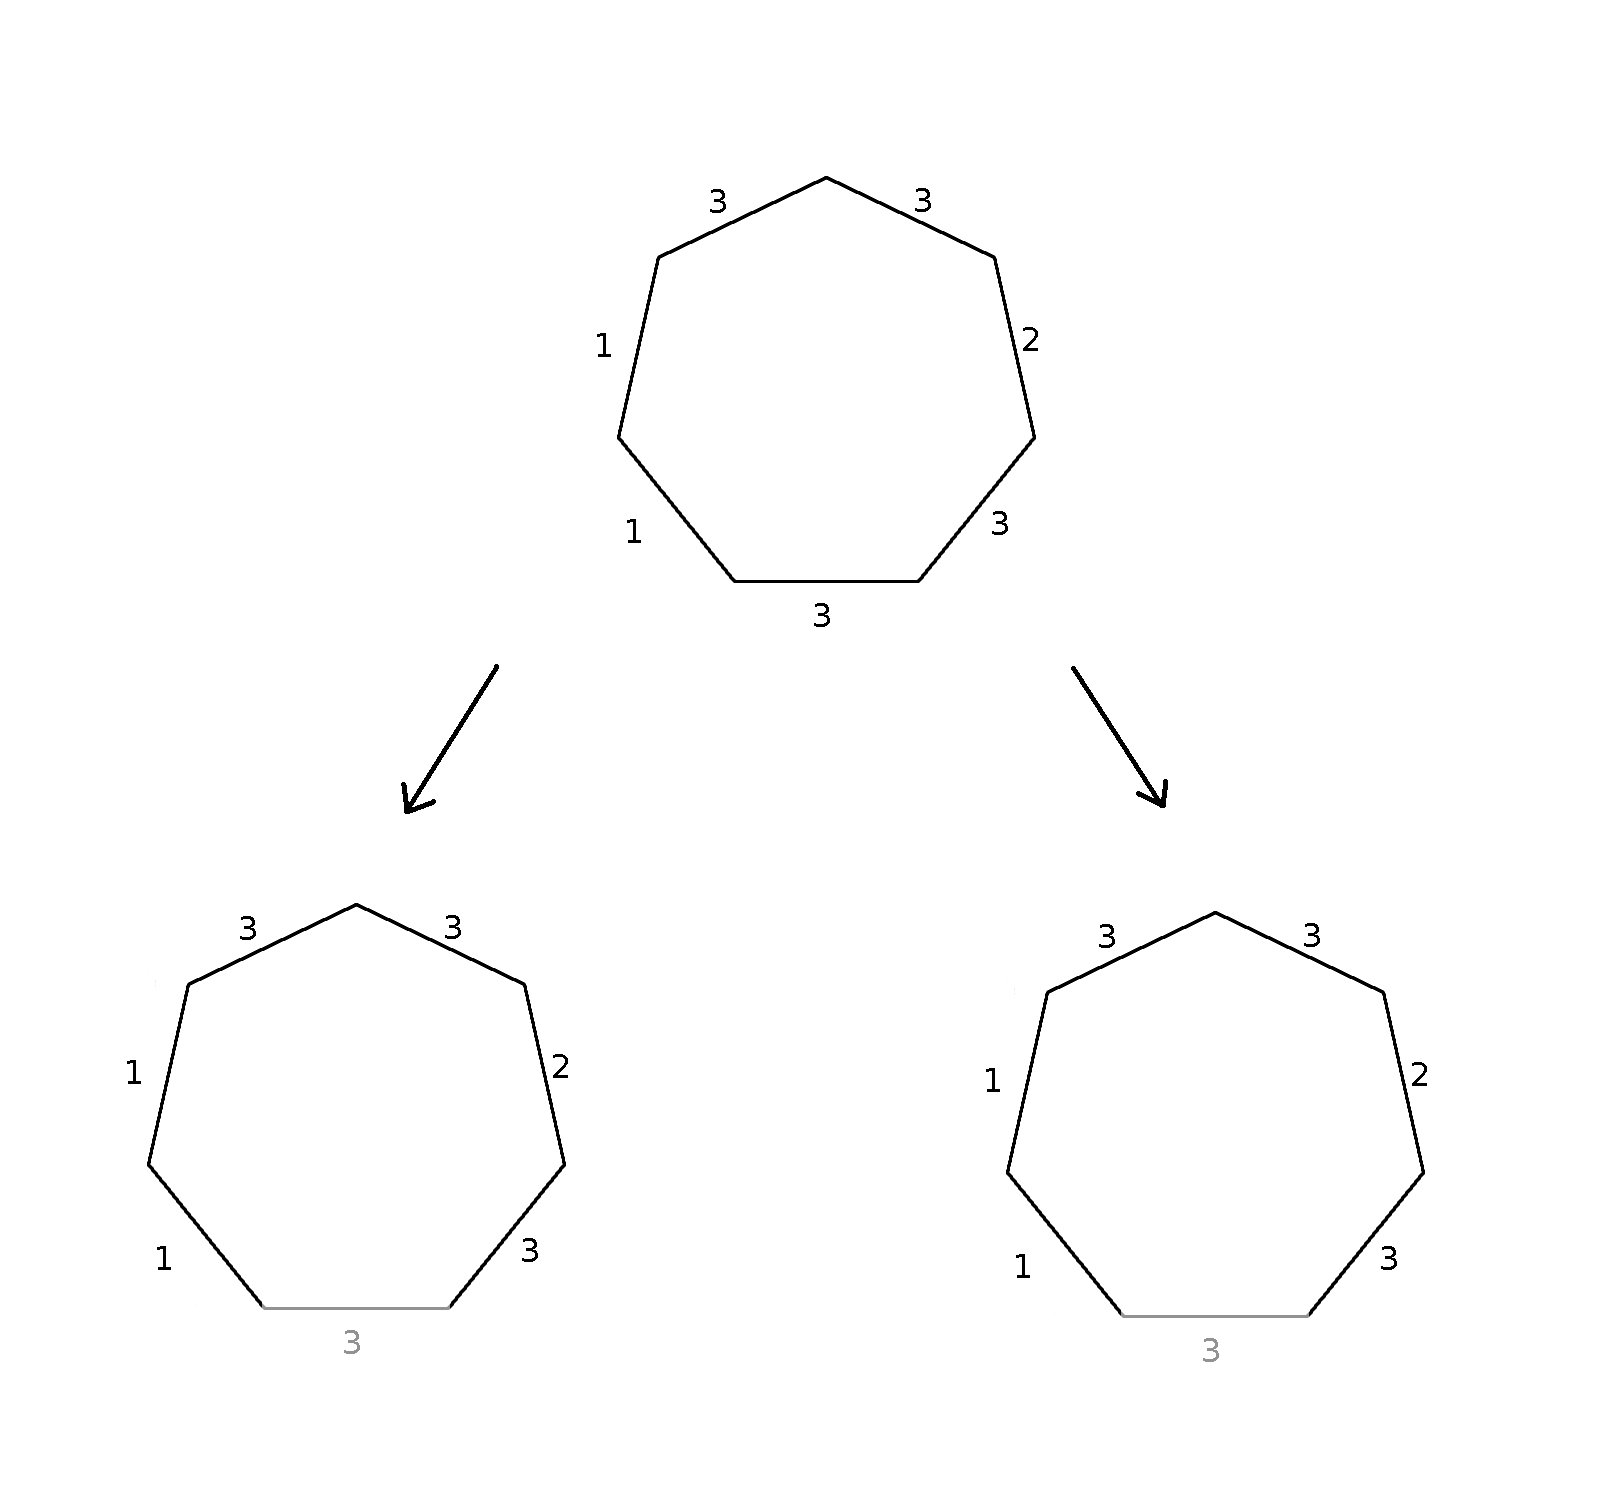
\includegraphics[width=0.7\textwidth]{imagenes/paso1y2.png}
\caption{Se toma la arista inferior y se bifurca entre utilizar la misma o no}
\end{center}
\end{figure}

\begin{figure}[H]
\centering
\subfloat[Derecha 1]{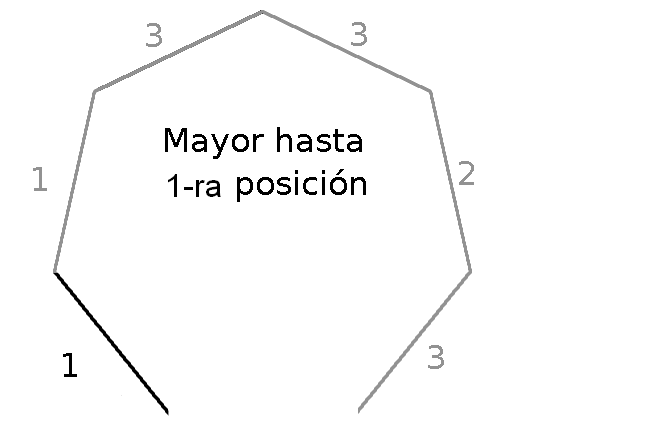
\includegraphics[width=0.3\textwidth]{imagenes/paso0b.PNG}}
\qquad
\subfloat[Izquierda 1]{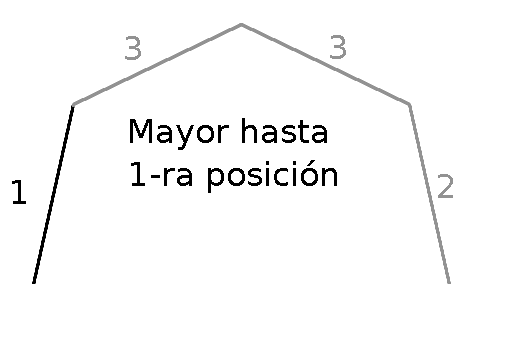
\includegraphics[width=0.3\textwidth]{imagenes/paso3a.png}}
\caption{Dos figuras en la misma linea}
\end{figure}

\begin{figure}[H]
\centering
\subfloat[Derecha 1]{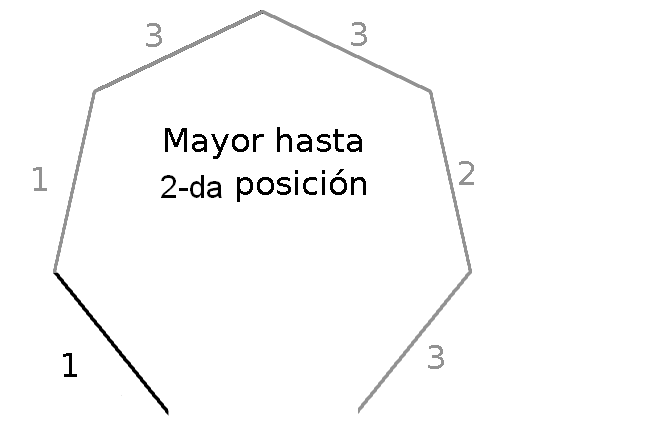
\includegraphics[width=0.3\textwidth]{imagenes/paso1b.PNG}}
\qquad
\subfloat[Izquierda 1]{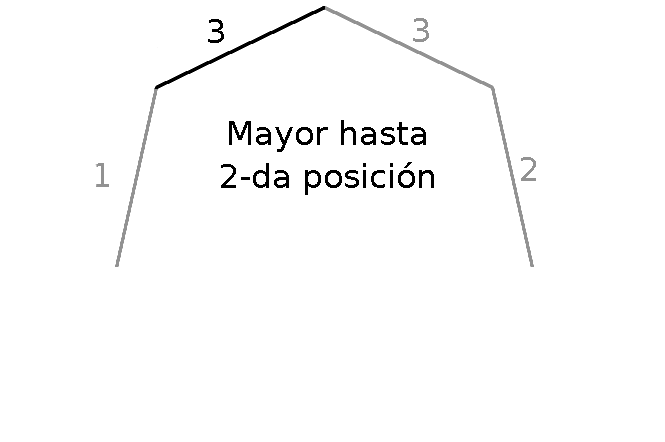
\includegraphics[width=0.3\textwidth]{imagenes/paso4a.png}}
\caption{Dos figuras en la misma linea}
\end{figure}

\begin{figure}[H]
\centering
\subfloat[Derecha 1]{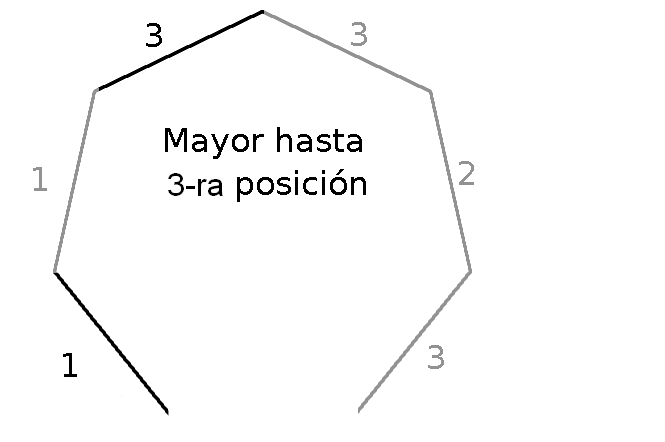
\includegraphics[width=0.3\textwidth]{imagenes/paso2b.PNG}}
\qquad
\subfloat[Izquierda 1]{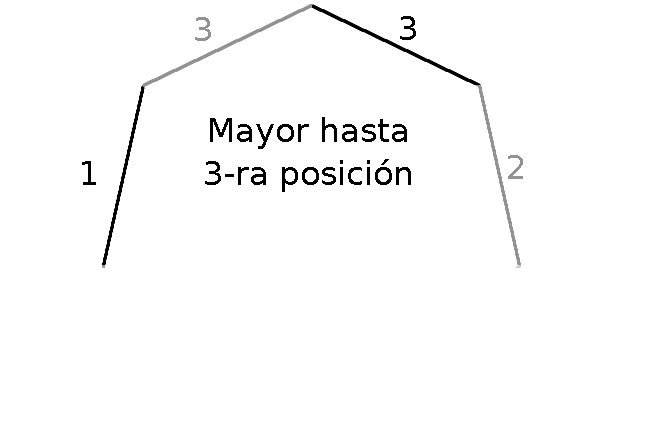
\includegraphics[width=0.3\textwidth]{imagenes/paso5a.png}}
\caption{camino a}
\end{figure}

\begin{figure}[H]
\centering
\subfloat[Derecha 1]{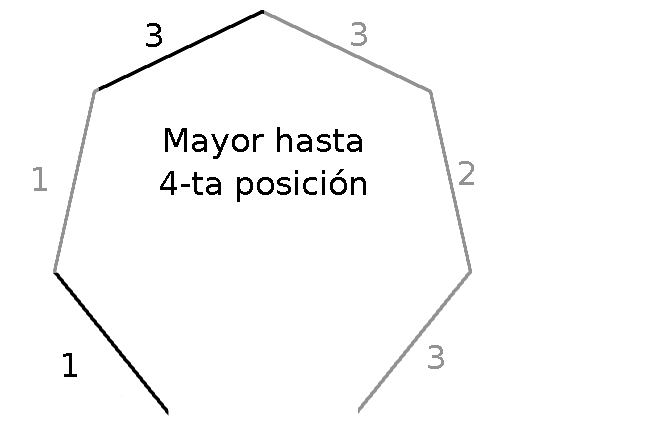
\includegraphics[width=0.3\textwidth]{imagenes/paso3b.png}}
\qquad
\subfloat[Izquierda 1]{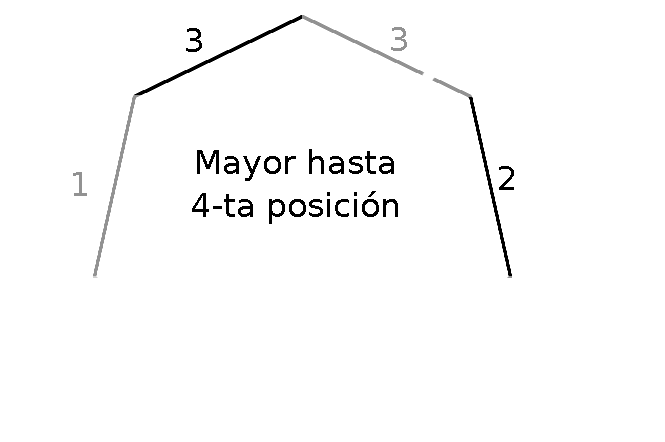
\includegraphics[width=0.3\textwidth]{imagenes/paso6a.png}}
\caption{fin de camino a}
\end{figure}

\begin{figure}[H]
\centering
\subfloat[Derecha 1]{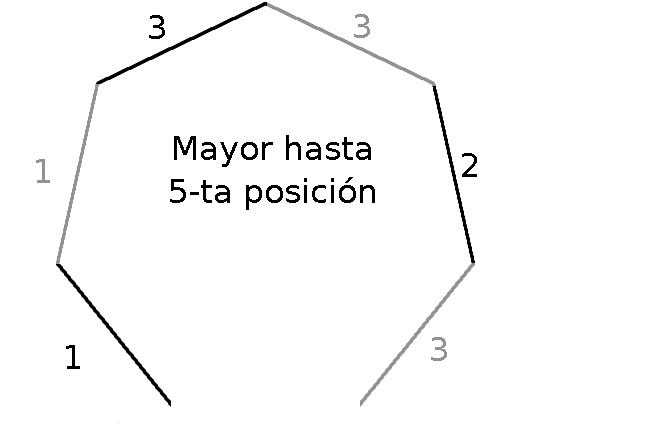
\includegraphics[width=0.3\textwidth]{imagenes/paso4b.png}}
\qquad
\subfloat[Izquierda 1]{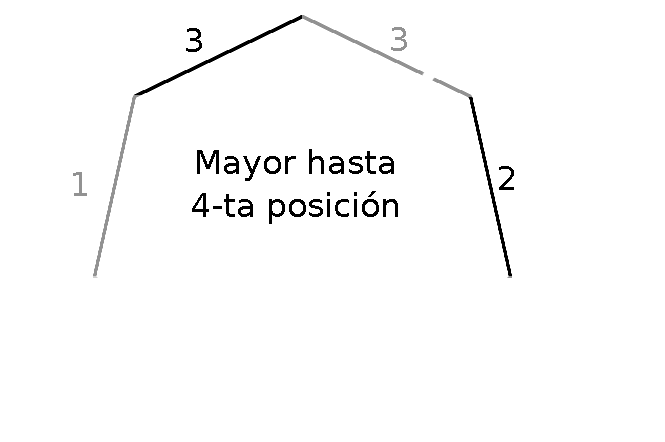
\includegraphics[width=0.3\textwidth]{imagenes/paso6a.png}}
\caption{fin de camino a}
\end{figure}

\begin{figure}[H]
\centering
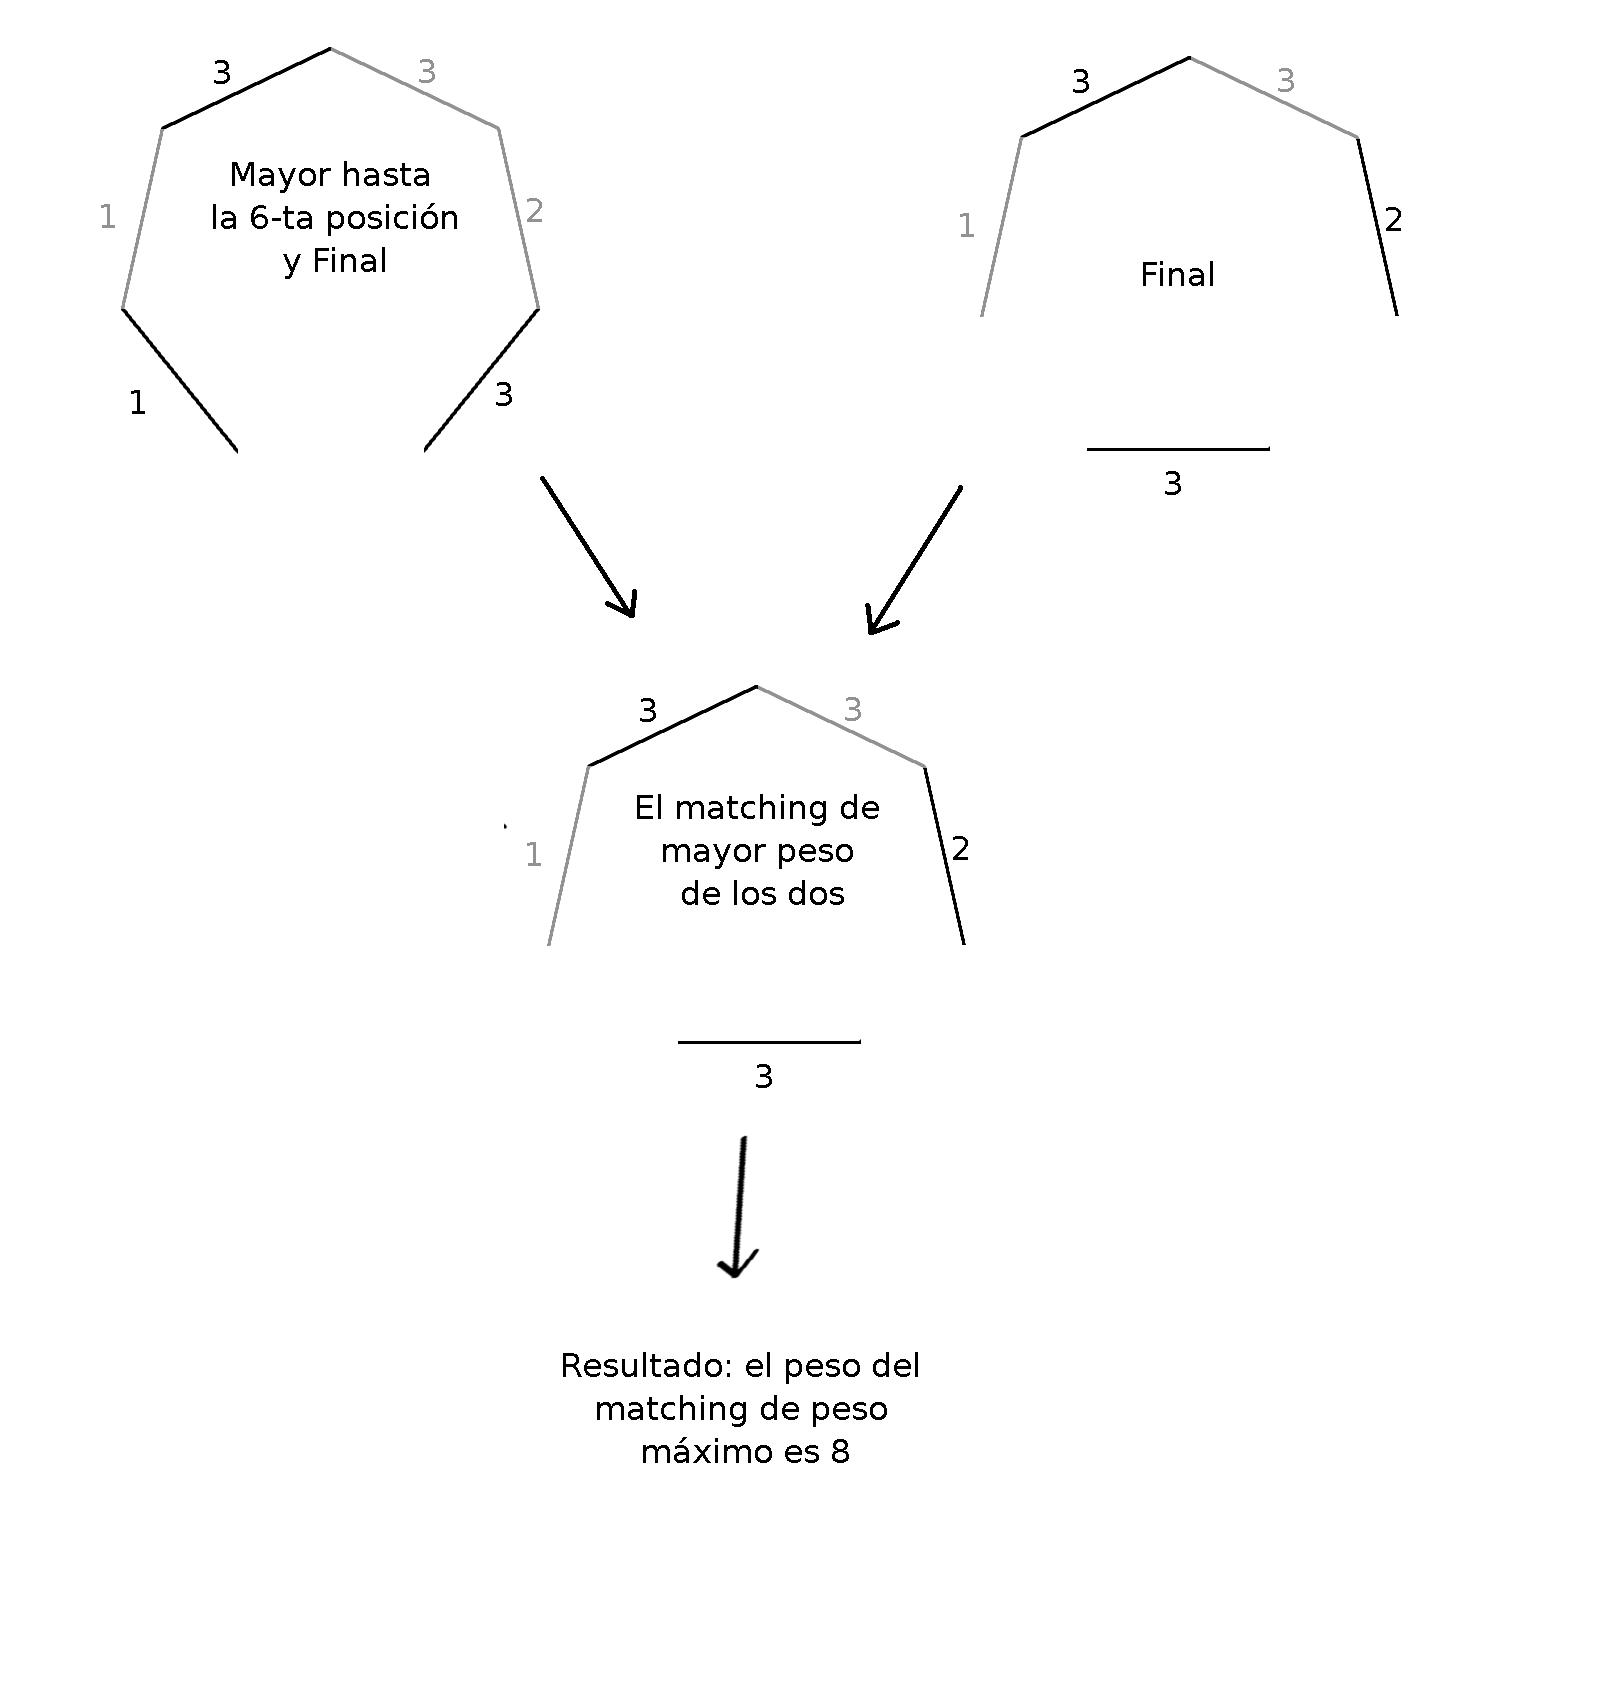
\includegraphics[width=0.7\textwidth]{imagenes/pasosFinales.png} 
\caption{union de los caminos}
\end{figure}

\section*{Demostraci\'on de correctitud}

Aca va la demostracion, Doc yo no entendi muy bien tu demo porque parece como que definis matching maximo posta de la misma manera que lo define nuestro algoritmo y nose, no digo que este mal, sino que me choca un toque, despues lo hablamos bien.


\section*{Complejidad}

Se analizar\'a la complejidad de este algoritmo en funci\'on del modelo uniforme.

En primer lugar, el algoritmo dise\~{n}ado toma una arista cualquiera, lo cual se ejecuta en un tiempo constante dado que los v\'ertices se encuentran en un vector de acceso indexado. Luego, se toman los dos vecinos que, dado que el grafo es un circuito simple, tambi\'en se los puede obtener en un tiempo constante. Luego, el algoritmo realiza una llamada a otro algoritmo que resuelve el matching m\'aximo sobre vectores. Por \'ultimo, se realiza una comparaci\'on entre los dos resultados arrojados por la rutina auxiliar para poder devolver el m\'aximo, sienda esta una operaci\'on tambi\'en de costo constante. Es por esto que la complejidad de este algoritmo esta regida entonces por la complejidad de la rutina auxiliar a la que hace referencia, ya que todas las demas operaciones toman un tiempo constante de ejecuci\'on.

Resulta necesario ver entonces la complejidad del algoritmo de matching m\'aximo sobre vectores.
Este algoritmo comienza realizando comparaciones del tama\~{n}o del vector para ver si el mismo se resuelve trivialmente. En todos estos casos los costos de las operaciones son constantes. Sin embargo, el peor caso, es que el vector pasado como par\'ametro contenga tres o m\'as elementos, por lo que la complejidad del algoritmo estar\'a dada por los costos de las operaciones en el caso de que el tama\~{n}o sea tres o m\'as.

En este caso, lo primero que se realiza son dos asignaciones y una comparaci\'on, lo cual toma tiempo constante. Luego, se realiza un ciclo tomando valores desde tres hasta n. Una vez dentro del ciclo, se realizan varias operaciones de tiempo constante, m\'as especificamente se realizan tres asignaciones, una suma y una comparaci\'on. Luego, al tener un ciclo que se ejecuta n-2 veces y sabiendo que dentro del ciclo las operaciones toman un tiempo constante, se puede aseverar que la ejecuci\'on de este ciclo ser\'a O(n). 

Por \'ultimo, dado que en este \'ultimo caso las operaciones son dos constantes y el ciclo mencionado, se puede asegurar que la complejidad total del algoritmo para encontrar el matching sobre un vector es O(n).

Finalmente, al ya haber mencionado que la complejidad del algoritmo principal se reg\'ia por la complejidad de la subrutina utilizada. Se puede ver que la complejidad de todo el algoritmo ser\'a lineal, es decir O(n). Es importante notar que para encontrar un matching m\'aximo, como m\'inimo hay que observar todas las aristas, por lo que la complejidad lineal resulta ser \'optima.

Tamanio de la entrada?!?!?! aca va algo de eso!?!? o ya esta bine asi??


\section*{An\'alisis de resultados}

Para analizar este algoritmo, se bas\'o el enfoque en dos aspectos diferentes. Por un lado, se encuentran los an\'alisis sobre la correctitud de la soluci\'on propuesta y, por otro lado, se encuentra el an\'alisis sobre el tiempo de ejecuci\'on para diferentes archivos de entrada, para poder realizar as\'i, una correlaci\'on entre el tiempo de ejecuci\'on y la complejidad te\'orica calculada anteriormente.

\subsection*{Casos de correctitud}
Con el fin de realizar una comprobaci\'on emp\'irica de la soluci\'on propuesta se genero un archivo de entrada con diez casos de prueba.
\begin{itemize}
\item Los primeros nueve casos de prueba, estan conformados por los entregados por la c\'atedra, teniendo de esta manera las soluciones reales para contrastar con las arrojadas por el algoritmo.
\item El \'ultimo caso de prueba esta conformado por un grafo de 30 aristas, con pesos de 1 a 30, ordenados consecutivamente. En este caso, se puede ver que el matching m\'aximo esta dado por tomar las aristas con valor par.
\end{itemize}

El an\'alisis en este tipo de casos se baso solamente en la correctitud de los mismos y no en el tiempo de ejecuci\'on debido a que son grafos de tama\~{n}os muy peque\~{n}os y el tiempo de ejecucion no sobrepasa los 2 microsegundos en ninguno de los casos.

Para todos los casos propuestos los resultados fueron satisfactorios al ser contrastados con la soluciones previamente obtenidas.

\subsection*{Casos para probar el tiempo de ejecuci\'on}
Para poder analizar como se comportaba el algoritmo en funci\'on del tama\~{n}o del grafo a procesar, se implemento un generador de ciclos simples al azar. El mismo se realiz\'o para que arrojase una salida con 500 grafos diferentes, el primero con 10000 aristas, el segundo con 10500 y as\'i sucesivamente. Una vez obtenidos los tiempos de ejecuci\'on de cada uno de estos casos, se procedi\'o a graficar los resultados para poder contrastar con la complejidad obtenida teoricamente.

A continuaci\'on se presenta un gr\'afico donde se encuentran simultaneamente los datos obtenidos y un ajuste lineal de los mismos.


\begin{figure}[H]
\centering
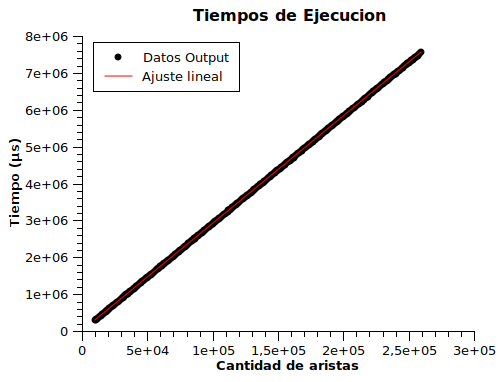
\includegraphics[width=0.7\textwidth]{imagenes/Resultados1.png} 
\caption{Grafico 1}
\end{figure}

Como se puede observar en el gr\'afico, los resultados fueron satisfactorios. El ajuste lineal arroj\'o un coeficiente de correlaci\'on de aproximadamente 0.99999, mostrando emp\'iricamente que la complejidad te\'orica calculada se condice con los tiempos reales de ejecuci\'on. 

\section*{Conclusiones}

Luego de obtener los resultados para el presente ejercicio, se concluyen varios puntos importantes:

\begin{itemize}
\item Si bien el problema de matching es de gran complejidad algor\'itmica, es necesario explotar el hecho de que solo se debe realizar sobre ciclos simples. El hecho de haber explotado esta caracter\'istica de los grafos presentes en la entrada del algoritmo, fue de gran importancia al momento de lograr un algoritmo eficiente que solo recorriese cada aristas una \'unica vez.
\item Resulta de gran importancia pensar diferentes variantes para el algoritmo con el fin de encontrar la versi\'on m\'as eficiente. Durante el dise\~{n}o del algoritmo se pens\'o tanto una estrategia de divide and conquer, como una estrategia de programaci\'on din\'amica. Si bien ambas resolv\'ian el problema satisfactoriamente dada que la idea era basicamente la misma solo que se invert\'ia el orden del recorrido del grafo, cabe destacar como la simple mejora de recorrer desde el primer elemento hasta el \'ultimo trajo la gran ventaja de preguntar por cada configuraci\'on de aristas una sola vez, generando as\'i un algoritmo de orden lineal, a diferencia del algoritmo exponencial obtenido por divide and conquer.
\item La complejidad te\'orica calculada se pudo ver reflejada en los casos de prueba propuestos. Se cree que la calidad del ajuste lineal que se consiguio se debi\'o a que el algoritmo no presenta mejores o peores casos; es decir, para todo grafo posible el algoritmo debe recorrer exactamente la misma cantidad de veces cada arista. De esta manera, los casos de prueba creados aleatoriamente no pueden ser beneficiados por el azar en ning\'un caso, generando una casi perfecta correlaci\'on lineal en funci\'on de la cantidad de aristas.
\end{itemize}



\begin{center}
\item \section*{Ejercicio 2: Se inunda la isla}
\end{center}

\section*{Introducci\'on}
En este ejercicio se pedia encontrar el area que no se inunde en una isla plana luego de ciertas condiciones.

En primer lugar, se tiene una isla que posee la misma altura en todos sus puntos, es por esto que si la marea sube la isla se inunda por completo. La soluci\'on para que las partes importantes de la isla no se inunde cuando sube la marea, es poner una serie de vallas rectangulares que no dejen pasar el agua hasta cierta altura. La idea ser\'ia entonces, colocando adecuadamente estas vallas, encerrar partes de la isla para que el agua no pueda entrar.

Aca se podria poner un dibujo de ejemplo de la isla con ciertas vallas o algo asi.

El problema consiste en, dado un conjunto de vallas y el nivel de la marea. Calcular cual es el area de la isla que no va a ser inundada.

\section*{Algoritmo}

A continuaci\'on se presenta una explicaci\'on al algoritmo propuesto como soluci\'on, seguido por su respectivo pseudoc\'odigo.

En primer lugar se observa que, por restricci\'on del problema, las vallas no pueden estar en cualquier lado, sino que su coordenada (x,y) del punto inferior izquierdo esta formada por x e y enteros. Asimismo, como la longitud de una valla tambien es entera, la coordenada del v\'ertice restante tambien ser\'a entera. De esta manera, podemos ver que la isla se puede pensar como una grilla de cuadrados de 1x1. Luego, esta grilla fue pensada como un grafo, donde cada cuadrado de la grilla es un nodo y las aristas estan dadas por la relaci\'on entre un cuadrado y sus 4 posibles vecinos. Para armar esta grilla, se calcularon los m\'inimos y m\'aximos valores de las vallas en x y en y, ya que por fuera de estos los cuadrados que pertenezcan a la isla se inundar\'an de todos modos (ya que no hay vallas que los cubran).

Al comenzar el algoritmo, todos los cuadrados estan relacionados con sus vecinos con aristas de peso 0. Esto quiere decir que si un cuadrado se inunda, los cuadrados que esten relacionados con ese por una arista de peso 0 tambien se va a inundar. 

Luego, se recorren todas las vallas dadas por el problema y se setean las nuevas relaciones entre los cuadrados, es decir, si existe una valla de altura 4 entre el nodo $v_1$ y el nodo $v_2$, lo que se hace es ponerle un peso de 4 a la arista que los relaciona. Indicando as\'i que solamente si la marea es mayor a 4, el agua pasara de ese $v_1$ a $v_2$ directamente.

Por \'ultimo, lo que se hace es crear una circunvalaci\'on de nodos que se inundan alrededor del grafo real y realizar BFS desde uno de estos (que seguro se inunda, por estar por fuera de las vallas) y contar cuantos nodos tiene la componente conexa que el BFS recorre por completo. Cabe destacar, este BFS toma que un nodo es vecino de otro si la arista que los une tiene peso menor a la marea, sino se puede decir que la valla es efectiva entre esos dos nodos y no hay inundaci\'on de uno hacia el otro. Una vez obtenida la cantidad total de nodos dados por el recorrido en anchura, resta el \'ultimo paso que es realizar la sustracci\'on entre los nodos totales de la grilla, y los nodos inundados; obteniendo as\'i, la cantidad total de nodos que no fueron inundados gracias a la protecci\'on de las vallas. Por \'ultimo, como cada nodo representa un cuadrado de \'area 1, la cantidad de nodos no alcanzados por el BFS es igual al \'area no inundada.

A continuaci\'on se presenta el pseudoc\'odigo del algoritmo recientemente explicado.

\begin{verbatim}
areaNoInundada(){
	vector vallas;
	leer(vallas)
	maxmin(vallas)
	matriz nodo[alto][ancho];
	seteamosMatriz(matriz)
	int inundadas  <- bfsContador(matriz)
	return (ancho*alto - inundadas)
}
\end{verbatim}



\begin{itemize}
\item leer(vallas): Carga en el vector vallas todas las provenientes del input.

\item maxmin(vallas): Setea ciertas variables con el tama\~no m\'aximo que tendrá la isla delimitada por las vallas mas externas.

\item seteamosMatriz(matriz): Usando las variables seteadas por maxmin crea un grafo (representado con una matriz) donde establece 4 relaciones por nodo (con sus vecinos) donde el peso del a arista es la altura de la valla que debe atravesar.

\item bfsContador(matriz): Recorre el grafo usando bfs, por cada nodo que visita suma uno a una variable que al final devuelve. Recorre todos los nodos que se inundan dado q son los que se relacionan (si la marea supera el peso de las aristas). De este modo al finalizar obtenemos cuantos nodos visitamos coincidiendo con cuantos nodos se inundan.
\end{itemize}

\begin{figure}[H]
\centering
\subfloat[Derecha 1]{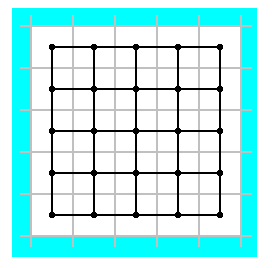
\includegraphics[width=0.3\textwidth]{imagenes/grafSinVallas.png}}
\qquad
\subfloat[Izquierda 1]{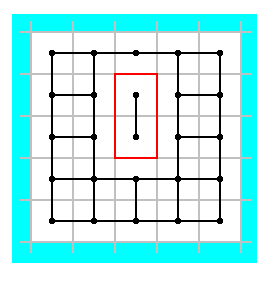
\includegraphics[width=0.3\textwidth]{imagenes/grafConVallas.png}}
\caption{fin de camino a}
\end{figure}

\begin{figure}[H]
\centering
\subfloat[Derecha 1]{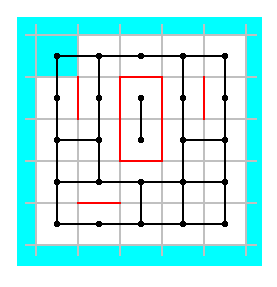
\includegraphics[width=0.2\textwidth]{imagenes/inundPaso1.png}}
\qquad
\subfloat[Izquierda 1]{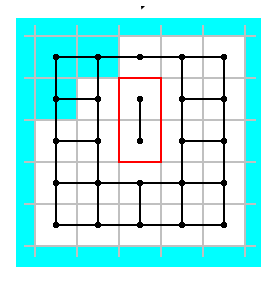
\includegraphics[width=0.2\textwidth]{imagenes/inundPaso2.png}}
\qquad
\subfloat[mas izq]{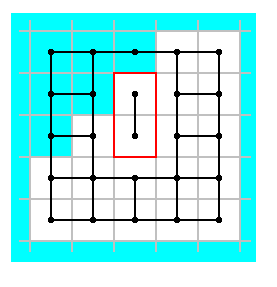
\includegraphics[width=0.2\textwidth]{imagenes/inundPaso3.png}}
\caption{fin de camino a}
\end{figure}

\begin{figure}[H]
\centering
\subfloat[Derecha 1]{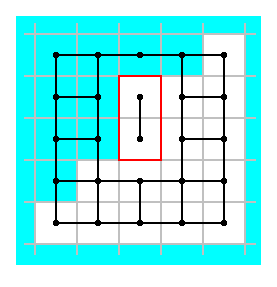
\includegraphics[width=0.2\textwidth]{imagenes/inundPaso4.png}}
\qquad
\subfloat[Izquierda 1]{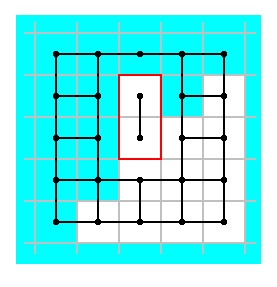
\includegraphics[width=0.2\textwidth]{imagenes/inundPaso5.png}}
\qquad
\subfloat[mas izq]{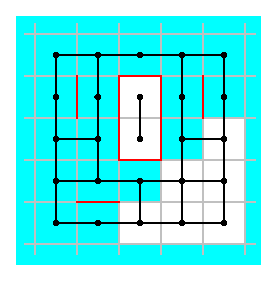
\includegraphics[width=0.2\textwidth]{imagenes/inundPaso6.png}}
\caption{fin de camino a}
\end{figure}

\begin{figure}[H]
\centering
\subfloat[Derecha 1]{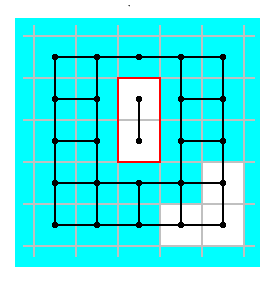
\includegraphics[width=0.2\textwidth]{imagenes/inundPaso7.png}}
\qquad
\subfloat[Izquierda 1]{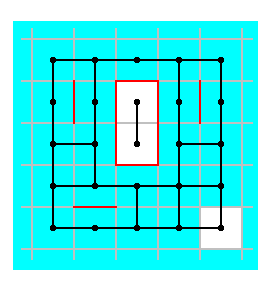
\includegraphics[width=0.2\textwidth]{imagenes/inundPaso8.png}}
\qquad
\subfloat[mas izq]{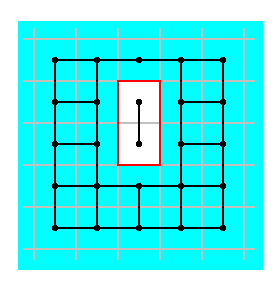
\includegraphics[width=0.2\textwidth]{imagenes/inundPasoFinal.png}}
\caption{fin de camino a}
\end{figure}


\section*{Complejidad}
Para analizar la complejidad se utiliz\'o el modelo uniforme. En este modelo el an\'alisis no esta centrado en el tama\~{n}o de los operandos, por lo que el tiempo de ejecuci\'on de cada operaci\'on se considera constante.

Si tomamos como tama\~no de entrada la cantidad de vallas (CV en adelante), y como sabemos que estas no se solapan en m\'as de un punto, podemos acotar por arriba a la cantidad de vallas, por un m\'ultiplo de la cantidad de nodos, si bien acotar las vallas por cuatro veces la cantidad de nodos resulta una cota grosera ya que se estan contando muchas vallas varias veces, la cota resulta util para poder enfocar el an\'alisis del algoritmo simplemente a la cantidad total de nodos; es decir, a la cantidad de casillas en la cuadr\'icula.

 
En primer lugar, la funci\'on maxmin, busca m\'aximos y m\'inimos en un vector de vallas linealmente, por lo cual es de orden O(CV) ya que se recorre todo el vector de vallas una vez.

En segundo lugar, se realiza el seteo de toda la matriz mediante la informaci\'on entregada por las vallas, en esta rutina se itera sobre todas las vallas y se setean las relaciones entre los nodos a partir de las alturas de las vallas pasadas como par\'ametro. En el peor de los casos, se tienen que setear las cuatro relaciones para cada uno de los nodos de la grilla. Como acceder al nodo se realiza en tiempo constante, y luego hacer los cuatros posibles cambios tambien se realiza en tiempo constante, esta rutina posee una complejidad de O(n) siendo n la cantidad de nodos de la grilla, ya que se realiza un ciclo sobre todos ellos, mientras que en cada iteraci\'on se realizan operaciones de complejidad O(1).

En \'ultimo lugar, lo que se hace es realizar un BFS para lograr identificar la cantidad de nodos de la componente conexa que se inunda. La rutina de BFS tiene una complejidad de O(n+m) siendo n la cantidad de nodos del grafo, y m la cantidad de aristas del mismo. Sin embargo, en este caso podemos acotar m por 4*n, ya que en el peor de los casos, cada nodo posee 4 vecinos. Luego, la complejidad de BFS en este caso es O(n).

En resumen, se realizan tres rutinas, la primera tiene una complejidad O(CV) que ya se mencion\'o que se puede acotar por O(n); luego, se realizan otras dos rutinas que ambas tiene complejidad O(n). Entonces, la complejidad total del algoritmo, es O(n), siendo n la cantidad de nodos del grafo que representa la isla. Cabe destacar que esta complejidad es an\'aloga a O(S), siendo S el \'area del rect\'angulo donde se puede inscribir la isla, ya que si bien el algoritmo agrega una fila y una columna O((altura+1)*(ancho+1)) = O(altura*ancho) = O(S).

\section*{An\'alisis de resultados}
Para analizar el funcionamiento del algoritmo propuesto como soluci\'on del problema, se realizaron dos tipos diferentes de casos de pruebas. Por un lado, se intento probar la correctitud del algoritmo mediante algunos casos de prueba de tama\~{n}o considerablemente peque\~{n}o, con el objetivo de poder contrastar las soluciones arrojadas por el algoritmo con las soluciones que se obtienen manualmente al poder visualizar la isla con las vallas correspondientes. Por otro lado, se intento constratar la complejidad te\'orica con el comportamiento real del algoritmo creando varias instancias de tama\~{n}os considerablemente grandes.

\subsection*{Casos de Correctitud}
Para analizar la correctitud del algoritmo, se utilizaron los siguientes casos de prueba:
\begin{itemize}
\item En primer lugar, se utilizaron los casos de prueba entregados por la c\'atedra. Los mismos constan de 6 islas con diferentes configuraciones de vallas.
\item Por otro lado, se genearon 9 islas tambi\'en con diferentes configuraciones de las vallas, de manera que los resultados de las mismas se pudiesen verificar manualmente.
\end{itemize}

Cabe destacar que todos los resultados obtenidos se contrastaron satisfactoriamente con los resultados esperados, tantos los entregados por la c\'atedra, como los obtenidos manualmente.

En este tipo de casos, solamente se menciona como fue el comportamiento del algoritmo en cuanto a la correctitud y no en cuanto al tiempo de ejecucion debido a que, en primer lugar, los tama\~{n}os de los grafos que represetan las islas son muy chicos como para obtener tiempos de ejecuci\'on representativos; y, por otro lado, las islas utilizadas poseen diferentes n\'umeros de vallas, lo que traer\'ia fluctuaciones en los tiempos de ejecuci\'on en caso de querer ser analizados.

\subsection*{Casos para probar el tiempo de ejecuci\'on}
Como se explic\'o en la secci\'on correspondiente, la complejidad de este algoritmo es lineal respecto de la cantidad de nodos del grafo que representa al rect\'angulo que inscribe a la isla. Es por esto, que para poder ver la relaci\'on entre la complejidad te\'orica y el comportamiento real del algoritmo, se crearon varias instacias de diferentes islas donde la cantidad de nodos creciera linealmente.

Se crearon 500 casos de prueba donde se mantuvieron ciertas caracter\'isticas invariantes para poder crear instancias comparables, mientras que el \'unico par\'ametro que se vari\'o fue la altura total del rect\'angulo en cuesti\'on.
Los casos de prueba se realizaron de la siguiente manera:
\begin{itemize}
\item Todos los casos tienen la marea de nivel 3.
\item Todos los casos poseen 8 vallas en total, todas de altura 4. Cuatro de las vallas se encuentran dentro del rect\'angulo encerrando un area no inundable de 1*2, con el simple objetivo de poseer un area no inundable.
\item De las otras 4 vallas, 3 son fijas, delimitando el ancho del rect\'angulo desde x igual a 1 hasta x igual a 10 y la restante delimita el borde inferior en y igual a 1.
\item La valla restante es la que se va modificando para generar instacias cada vez m\'as grandes. Comienza en el primer caso delimitando el borde superior en y igual a 10000, y luego va subiendo este l\'imite 500 unidades por cada caso.
\end{itemize}

Por lo explicado anteriormente, se puede ver que las islas son todas muy parecidas excepto por la cantidad de nodos en total que vari\'an desde 100000, subiendo de a 5000 nodos por cada caso. La idea de realizar islas muy parecidas excepto por la cantidad de nodos, fue que el seteo de vallas y sus respectivas relaciones fueran an\'alogas para todos los casos y que no fueran factor de fluctuaciones no deseadas en los tiempos de ejecuci\'on.

A continuaci\'on se presenta un gr\'afico donde se encuentran plasmados los tiempos de ejecuci\'on en cada caso, en funci\'on de la cantidad de nodos del grafo correspondiente.

\begin{figure}[H]
\centering
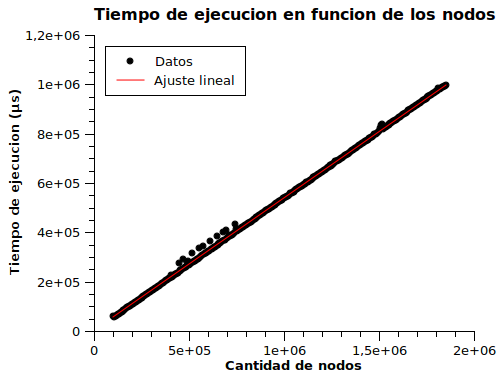
\includegraphics[width=0.7\textwidth]{imagenes/Resultados2.png} 
\caption{Grafico 1}
\end{figure}


Como se puede observar, las observaciones emp\'iricas de como funciona el algoritmo se condicen con la complejidad te\'orica
calculada anteriormente. Si bien se denotan la presencia de algunos \emph{outliers}, tambi\'en se puede observar claramente
como los datos estan relacionados por una funci\'on lineal tal como la complejidad te\'orica predicaba. Al realizar el ajuste lineal
se consigui\'o un ajuste con un coeficiente de correlaci\'on de aproximadamente 0.999.

\section*{Conclusiones}
Luego de obtener los resultados pertinentes a los diferentes casos de prueba se concluye que:
\begin{itemize}
\item Es importante tener en cuenta varios modelos diferentes a la hora de dise\~{n}ar un algoritmo para resolver un problema
en particular, ya que si bien la idea de una inundaci\'on de una isla puede estar bastante alejada de un problema de grafos, lograr
esta correlaci\'on hizo que el problema se pudiese realizar con un buen orden de complejidad y minimizando bastante bien la cantidad de 
veces que se itera sobre las diferentes partes de la isla.
\item Resulta de gran importancia tener en cuenta algunos peque\~{n}os detalles de dise\~{n}o, ya que estos pueden ser muy
relevantes en el resultado final. Por ejemplo, en este algoritmo fue importante el hecho de agrandar la grilla una linea en cada direccion, 
de lo contrario la complejidad del mismo ubiese cambiado porque se tendr\'ia que haber realizado varios BFS.
\item La complejidad te\'orica calculada se pudo contrastar emp\'iricamente con los casos de prueba utilizados. Igualmente, 
cabe destacar que se presetaron algunos pocos outliers que se desconoce su origen, para todos los dem\'as datos, se puede ver que
el tiempo de ejecuci\'on aumenta linealmente en funci\'on de la cantidad de nodos.
\item Para poder analizar el tiempo de ejecuci\'on fue necesario buscar casos de prueba donde lo \'unico que variase fuera la cantidad de nodos,
si otro par\'ametro hubiese variado (la cantidad de vallas por ejemplo, o la disposici\'on de las mismas) el tiempo de ejecuci\'on 
podr\'ia haber fluctuado sin tener esta fluctuaci\'on una relaci\'on con la cantidad de nodos, efecto que no es deseado. 
\end{itemize}


\begin{center}
\item \section*{Ejercicio 3: Bernardo Armando Pandillas}
\end{center}

\section*{Introducci\'on}


En este problema lo que se quiere es, teniendo un conjunto de personas y sabiendo si se conocen entre s\'i, armar dos grupos de tres personas cada uno, un grupo en el cual las 3 personas se conozcan mutuamente, y otro grupo en el cual ninguno est\'e relacionado con otro.


En el caso que se pudieran armar varios grupos que cumplan con la restricci\'ones planteadas, los que se deben encontrar son los menores lexicogr\'aficamente, para cada uno de los dos casos. Es decir, si se representa cada grupo con una terna ordenada ascendentemente, la terna ser\'a menor que cualquier otra terna que represente a un grupo v\'alido.

Se considera que una terna es menor que otra si la primera componente de la primera terna es menor, o si es igual y la segunda de la misma es menor, o si tanto la primera como la segunda son iguales y la tercera es menor, en cada caso con respecto a la misma componente de la otra terna.
\begin{displaymath}
\left(a, b, c \right) < \left( d, e, f\right) \Leftrightarrow 
\left( a < d \right) \vee \left( a = d \wedge b < e \right) \vee \left( a = d \wedge b = e \wedge c < f \right)
\end{displaymath}


\section*{Algoritmo}

Para lograr el objetivo deseado se opt\'o por representar el problema mediante la utilizaci\'on de un grafo en donde cada v\'ertice del mismo representase a una persona diferentes, mientras que las aristas fuesen las encargadas de representar las relaciones de conocimiento, teniendo as\'i la presencia de una arista entre dos nodos diferentes si y solo si las personas representan por dichos nodos se conocen.


Una vez obtenido el grafo de relacion, lo que se busca es un clique de 3 nodos, ya que se puede ver que existe un clique de tres nodos si y s\'olo si las personas representadas por los nodos que est\'en en dicho clique se conocen todas entre s\'i. Ver Ap\'endice \ref{dem_clique}.


Encontrar un clique de 3 nodos, encontrar\'ia entonces las conformaciones posibles para el grupo Coppersmith. Luego, se necesita buscar como formar el grupo Winograd. Para encontrar este grupo de tres personas que no se conozcan entre s\'i, lo que se hizo fue resolver el mismo problema pero en el grafo complemento, ya que este nuevo grafo representa las no-relaciones entre las personas. Ver Ap\'endice \ref{dem_clique}.

Una vez demostrado que la extrapolaci\'on del modelo elegido es correcta para poder resolver el problema pedido, se aboca el algoritmo a encontrar un clique de tres nodos en el grafo.
Para encontrar el clique se realizan los siguiente pasos:

\begin{enumerate}
\item En primer lugar, se confecciona la matriz de adyacencias utilizando las relaciones entre las personas, en la cual el nodo i-\'esimo representa a la i-\'esima persona. A partir de aqui, se llamar\'a $A$ a esta matriz de adyacencia.
\item Luego, sea $C = A^3$, entonces se puede ver que $C$ tiene en la i-\'esima posici\'on de su diagonal la cantidad de caminos de longitud 3 desde el nodo i hasta el nodo i. \footnote{Te\'orica Algoritmos III} Esto justamente indica la presencia de un clique de 3 nodos dado que, en el caso especial de 3 nodos, un clique o un circuito es lo mismo.
\item Una vez que se puede conocer los nodos que estan en un circuito de 3 nodos mirando la diagonal, se busca en $C$ el m\'inimo i tal que $C_{i,i} \neq 0$, llam\'emoslo j. Si existe, entonces, el menor clique de 3 nodos contendr\'a a j. Si no fuera as\'i, entonces existe $k < j$ tal que $C_{k,k} \neq 0$, lo cual es un absurdo, ya que j es el m\'inimo i tal que $C_{i,i} \neq 0$. Si no existe, termina el algoritmo indic\'andolo de manera correspondiente que como no hay ninguna persona que este involucrada en un ciclo de 3 nodos, entonces no se puede armar el grupo Coppersmith.
\item Una vez obtenido el menor nodo que esta presente en un clique de 3 nodos, de todas las combinaciones posibles para los otros dos nodos, se elige la menor tal que los tres nodos forman un clique. En la implementaci\'on se optimiza esta ultima selecci\'on, evitando generar combinaciones que se sepa anticipadamente que no corresponden a un clique. De esta manera se obtuvo el grupo de tres personas que se conocen entre s\'i.
\item Por \'ultimo se obtiene el grafo complemento de $G$, y se realizan las mismas operaciones para obtener el grupo de tres personas que no se conocen entre s\'i, el grupo Winograd.
\end{enumerate}

\section*{Complejidad}

Para analizar la complejidad del algoritmo, se va ir analizando que se hace en cada paso, calculando la complejidad del mismo.

En primer lugar, se setea toda la matriz de adyacencias mediante la informaci\'on obtenida del caso pertinente. Lo que se hace es ir poniendo en cada posici\'on un 0 o un 1 seg\'un corresponda, es por esto que este paso es del orden de n cuadrado, siendo n la cantidad de nodos del grafo.

Luego, se obtiene $C = A^3$ utilizando el algoritmo de Strassen para realizar el producto de matrices. La cantidad de operaciones que realiza este algoritmo est\'a en $O\left(m^{log_2\left(7\right)}\right)$, para una matriz de $m$ filas y $m$ columnas.\footnote{Ver Brassard, p\'ag. 273.} En el caso de que el grafo tenga $n$ nodos, es necesario generar una matriz de $m \times m$, con $m \leq 2n$, ya que es necesario que $m$ sea una potencia de dos. De esta forma, la cantidad de operaciones para realizar el producto de matrices est\'a en $O\left(7 \times \left(n ^{log_2 \left( 7\right)} \right) \right) = O\left(n^{log_2\left(7\right)}\right)$.



Una vez obtenida la matriz elevada al cubo, es momento de buscar el m\'inimo elemento de la diagonal que sea distinto de 0. Se puede encontrar en $C$ el m\'inimo $i$ tal que $C_{i,i} \neq 0$ en $O\left(n\right)$ operaciones, ya que para cada posici\'on de la diagonal se realiza una cantidad constante de operaciones para verificar si en dicha posici\'on hay un cero. Para realizar esto, se recorre toda la diagonal que posee n elementos, cumpliendo as\'i con la complejidad dicha.

Luego de obtener el menor nodo que se encuentra en un clique, hay que generar todas las dem\'as combinaciones para ver cuales forman un clique. 
Al generar todas las combinaciones de dos nodos la cantidad de operaciones para obtener la menor est\'a en $O\left(n^2\right)$, ya que se requiere una cantidad constante de operaciones para generar cada combinaci\'on, verificar si es un clique y compararla con la menor hasta el momento.

Luego, al tener todos los c\'alculos realizados para la busqueda del grupo Coppersmith, se puede ver por todo lo antedicho que la operaci\'on predominante esta dada por la multiplicaci\'on de las matrices que se realiza en $O\left(m^{log_2\left(7\right)}\right)$, siendo esta la complejidad del algoritmo para toda esta primer parte.

Por \'ultimo se realizan las mismas operaciones sobre el grafo complemento. Para lo cual se invierte la matriz de adyacencias en $O \left( n^2 \right)$.


Entonces, como se puede ver, la complejidad computacional del algoritmo en el modelo uniforme est\'a dada por las operaciones correspondientes a la multiplicaci\'on de matrices, en $O \left( n^{log_2\left(7\right)} \right) $, ya que el resto del algoritmo tiene un orden menor. Como $log_2\left(7\right) < 2.9 $, el algoritmo realiza una cantidad de operaciones de un orden estrictamente menor a $O\left( n^3\right) $.




\section*{An\'alisis de resultados}
\section*{Conclusiones}

\section*{Ap\'endices}
\section{Demostraci\'on de correctitud del modelo}\label{dem_clique}

Para resolver el ejercicio 3 se opta por representarlo mediante un grafo.

Cada v\'ertice del grafo representa a una persona diferente y dos v\'ertices est\'an unidos si y s\'olo si las personas se conocen.


A continuaci\'on se demuestra que existe un clique de tres nodos en el grafo que modela el problema si y s\'olo si las personas representadas por los nodos que est\'en en dicho clique se conocen todas entre s\'i. Luego se demuestra que existe un clique de tres nodos en el complemento del grafo planteado si y s\'olo si las personas representadas por los nodos que est\'en en dicho clique no se conocen entre s\'i.

Sea $G = \left( V, E \right)$ el grafo con el que modelamos el problema. Sea $ C = \left( \left\lbrace v_a, v_b,v_c \right\rbrace, E_c \right) $ un clique de tres nodos donde C es subgrafo de G y donde $v_a$ representa a la persona $a$, $v_b$ a la persona $b$ y $v_c$ a la persona $c$. Como $\left( v_a, v_b \right) \in E $, $a$ conoce a $b$. Tambi\'en $\left(v_b,v_c\right) \in E$, por lo que $b$ conoce a $c$. Por \'ultimo como $\left(v_c,v_a\right) \in E$, $c$ conoce a $a$. Por lo tanto las personas representadas por los nodos que est\'an en un clique de tres nodos se conocen entre s\'i de a pares.


A su vez, si tres personas, llam\'emoslas $a$, $b$ y $c$, se conocen entre s\'i de a pares, existe un clique de tres nodos que contiene a los nodos que las representan. 


Sea $ G = \left( V, E \right) $ el grafo con el que modelamos el problema. Sean $v_a, v_b, v_c$ los nodos que las representan, como $a$ conoce a $b$, $\left( v_a,v_b \right) \in E $. Como $b$ conoce a $c$, $ \left(v_b, v_c \right) \in E$. Como tambi\'en $c$ conoce a $a$, $ \left( v_c, v_a \right) \in E$, por lo tanto $\left( \left\lbrace v_a, v_b, v_c \right\rbrace, \left\lbrace  \left(v_a,v_b\right) , \left( v_b,v_c\right), \left( v_c, v_a\right) \right\rbrace\right)$ es un clique de 3 nodos subgrafo de G.


Resta demostrar que existe un clique de tres nodos en el complemento del grafo planteado si y s\'olo si las personas representadas por los nodos que est\'en en dicho clique no se conocen entre s\'i.


Llamemos $G' = \left( V', E' \right)$ al complemento de $G$.  Sea $ C = \left( \left\lbrace v_a, v_b,v_c \right\rbrace, E' \right) $ un clique de tres nodos donde C es subgrafo de G y donde $v_a$ representa a la persona $a$, $v_b$ a la persona $b$ y $v_c$ a la persona $c$. Como $\left( v_a,v_b\right) \in E'$, $a$ y $b$ no se conocen. Tambi\'en $\left( v_b,v_c\right) \in E'$, por lo que $b$ y $c$ no se conocen. Por \'ultimo $\left( v_c,v_a\right) \in E'$, y por lo tanto $c$ y $a$ no se conocen. Luego $a$, $b$, y $c$ forman un grupo de tres personas que no se conocen.



Rec\'iprocamente, si sabemos que $a$, $b$ y $c$ forman un grupo de tres personas que no se conocen entre s\'i, y sean $v_a, v_b, v_c$ los nodos que las representan, entonces como $a$ y $b$ no se conocen, $\left(v_a,v_b\right) \in E'$. Tampoco $b$ y $c$ se conocen, por lo que $\left(v_b,v_c\right) \in E'$. Por \'ultimo $c$ y $a$ no se conocen, por lo cual $\left(v_c,v_a\right) \in E'$. Luego $\left( \left\lbrace v_a, v_b, v_c \right\rbrace, \left\lbrace  \left(v_a,v_b\right) , \left( v_b,v_c\right), \left( v_c, v_a\right) \right\rbrace\right)$ es un clique de tres, subgrafo de $G'$.

\end{document}
